
\section{Additional Results}

\subsection{Remaining Results on EuRoC, TartanAirv2, and KITTI}
\label{sec:macvo:AdditionalResults}

See \tref{tab:EuRoCEven}, \tref{tab: TartanAirEasy}, and \tref{tab: KITTI Odd} for data.

\begin{table*}[ht]
\centering
\captionsetup{font=small}
\caption{Performance comparison of different methods on the EuRoC Dataset. Only even-ordered trajectory is shown here, see \tref{tab:EuRoCOdd} for the remaining results.}
\resizebox{\textwidth}{!}{
\begin{tabular}{lcccccccccccc}
\toprule
 Trajectory & \multicolumn{2}{c}{{MH02}} & \multicolumn{2}{c}{{MH04}} & \multicolumn{2}{c}{{V101}} & \multicolumn{2}{c}{V103} & \multicolumn{2}{c}{V202}\\
\cmidrule{2-11}
   &  $t_{\mathrm{rel}}$ & $r_{\mathrm{rel}}$ & $t_{\mathrm{rel}}$ & $r_{\mathrm{rel}}$ & $t_{\mathrm{rel}}$ & $r_{\mathrm{rel}}$ & $t_{\mathrm{rel}}$ & $r_{\mathrm{rel}}$ & $t_{\mathrm{rel}}$ & $r_{\mathrm{rel}}$\\
\midrule
\textbf{SLAM} \\
\hspace{3mm} \stereoicon~ORB-SLAM 3                & 0.0036 & 0.0495   &  0.0061  & 0.0501   &  0.0049  & 0.0888   &  0.0137  & 0.2669   &  0.0090  & 0.1528\\
\hspace{3mm} \stereoicon~DROID-SLAM$^\star$         & \textbf{0.0012} & \textbf{0.0169} & 0.0031   & \textbf{0.0224} & \textbf{0.0024} & \underline{0.0314} & 0.0036 & \underline{0.0642} & \textbf{0.0017} & \textbf{0.0399}\\
\hspace{3mm} \monoicon~MASt3R-SLAM$^{\star}$ & 0.0138 & 0.5493 & 0.0274 & 0.8890 & 0.0130 & 0.5808 & 0.0383 & 1.3178 & 0.0334 & 0.6818 \\
\midrule
\textbf{VO} \\
\hspace{3mm} \monoicon~TartanVO$^{\star}$  & 0.0172 & 0.0621 & 0.0213 & 0.0681 & 0.0124 & 0.0756 & 0.0263 & 0.1552 & 0.0171 & 0.1251\\
\hspace{3mm} \stereoicon~TartanVO                  & 0.0289 & 0.5037 & 0.0501 & 0.5400 & 0.0224 & 0.5322 & 0.0351 & 1.3127 & 0.0361 & 1.1607\\
\hspace{3mm} \stereoicon~iSLAM-VO                   & 0.0041 & 0.0620 & 0.0082 & 0.0682 & 0.0041 & 0.0756 & 0.0088 & 0.1554 & 0.0078 & 0.1252\\
\hspace{3mm} \monoicon~DPVO$^{\star}$      & 0.0014 & 0.0212 & \underline{0.0029} & \underline{0.0264} & \underline{0.0026} & 0.0405   & \underline{0.0033} & 0.0662   & 0.0022 & 0.0493\\
% \midrule
\rowcolor{ourgray}
\hspace{3mm} \stereoicon~\textbf{Ours}                           & \underline{0.0013} & \underline{0.0199} & \textbf{0.0028} & 0.0273   & \textbf{0.0024} & \textbf{0.0304} & \textbf{0.0032} & \textbf{0.058} & \underline{0.0018} & \underline{0.0406}\\
\bottomrule
\multicolumn{10}{l}{
\monoicon \hspace{.5mm} Monocular method.
\quad
\stereoicon \hspace{.5mm} Stereo method.
\quad
$^\star$ Scale-aligned with ground truth.} \\
\end{tabular}
}
\label{tab:EuRoCEven}
\end{table*}


% % \begin{table*}[htbp]
% % \centering

% % {\fontsize{8}{9}\selectfont \textbf{Relative Position Error (RPE)}}\\
% % \resizebox{\linewidth}{!}{\begin{tabular}{lccccccccccccccc}
% % \toprule
% % Traj. & E00 & E01 & E02 & E03 & E04 & E05 & E06 & E07 & E08 & E09 & E10 & E11 & E12 & E13 \\
% % \midrule
% % ORB-SLAM3           & 0.205 & - & - & - & - & 0.532 & - & - & - & - & - & - & - & -\\
% % DPVO$^{\star\dagger}$        & \underline{0.007} & 0.035          & \textbf{0.013} & 1.154          & 0.24           & 0.015          & \underline{0.012} & 0.027          & 0.033          & 0.302          & \underline{0.014} & 0.026          & 0.323          & 0.101          \\
% % DROID-SLAM$^\star$  & \textbf{0.003} & \textbf{0.02}  & 0.04           & \textbf{0.006} & \textbf{0.029} & \textbf{0.004} & \textbf{0.005} & \textbf{0.003} & \textbf{0.015} & \textbf{0.011} & \textbf{0.007} & \textbf{0.002} & \textbf{0.013} & \textbf{0.003} \\
% % iSLAM               & 0.136          & 0.177          & 0.204          & 0.176          & 0.157          & 0.141          & 0.126          & 0.124          & 0.139          & 0.148          & 0.184          & 0.279          & 0.493          & 0.104          \\
% % TartanVO$^{\star\dagger}$ & 0.426          & 0.381          & 0.924          & 0.373          & 0.884          & 0.471          & 0.466          & 0.44           & 0.641          & 0.422          & 0.399          & 0.687          & 0.85           & 1.429          \\
% % TartanVO         & 0.082          & 0.235          & 0.124          & 0.142          & 0.167          & 0.11           & 0.111          & 0.083          & 0.106          & 0.114          & 0.152          & 0.073          & 0.117          & 0.092          \\
% % \midrule
% % \textbf{Ours}       & 0.022          & \underline{0.028} & \underline{0.015} & \underline{0.04} & \underline{0.063} & \underline{0.012} & 0.013          & \underline{0.02} & \underline{0.026} & \underline{0.022} & 0.024          & \underline{0.01} & \underline{0.039} & \underline{0.035} \\
% % \bottomrule
% % \multicolumn{10}{l}{$^\star$ The estimated sequence is scale-aligned with ground truth}\\
% % \multicolumn{10}{l}{\small{$^\dagger$ Monocular method.}}
% % \end{tabular}}

% % \vspace{5mm}

% % {\fontsize{8}{9}\selectfont \textbf{Relative Orientation Error (ROE)}}\\
% % \resizebox{\linewidth}{!}{\begin{tabular}{lccccccccccccccc}
% % \toprule
% % Traj. & E00 & E01 & E02 & E03 & E04 & E05 & E06 & E07 & E08 & E09 & E10 & E11 & E12 & E13 \\
% % \midrule
% % ORB-SLAM3           & 0.148 & - & - & - & - & 0.149 & - & - & - & - & - & - & - & -\\
% % DPVO$^{\star\dagger}$ & \textbf{0.001} & \textbf{0.001} & \textbf{0.002} & 0.021          & \underline{0.019} & \textbf{0.001} & \textbf{0.001} & \underline{0.003} & \textbf{0.002} & 0.009          & \textbf{0.001} & \textbf{0.001} & \underline{0.005} & \underline{0.009} \\
% % DROID-SLAM$^\star$  & \textbf{0.001} & \textbf{0.001} & \textbf{0.002} & \textbf{0.001} & \textbf{0.004} & \textbf{0.001} & \textbf{0.001} & \textbf{0.001} & \textbf{0.002} & \textbf{0.001} & \textbf{0.001} & \textbf{0.001} & \textbf{0.003} & \textbf{0.001} \\
% % iSLAM               & 0.028          & 0.027          & 0.04           & 0.02           & 0.024          & 0.023          & 0.019          & 0.02           & 0.023          & 0.021          & 0.018          & 0.034          & 0.063          & 0.026          \\
% % TartanVO$^{\star\dagger}$ & 0.017          & 0.054          & 0.043          & 0.05           & 0.101          & 0.062          & 0.044          & 0.03           & 0.071          & 0.028          & 0.023          & 0.054          & 0.057          & 0.124          \\
% % TartanVO            & 0.018          & 0.014          & 0.021          & 0.026          & 0.026          & 0.018          & 0.012          & 0.027          & 0.012          & 0.012          & 0.02           & 0.017          & 0.037          & 0.024          \\
% % \midrule
% % \textbf{Ours} & \underline{0.006} & \underline{0.003} & \underline{0.004} & \underline{0.01} & 0.022          & \underline{0.003} & \underline{0.002} & 0.008          & \underline{0.005} & \underline{0.004} & \underline{0.004} & \underline{0.002} & 0.017          & 0.012          \\
% % \bottomrule
% % \multicolumn{10}{l}{$^\star$ The estimated sequence is scale-aligned with ground truth}\\
% % \multicolumn{10}{l}{\small{$^\dagger$ Monocular method.}}
% % \end{tabular}}
% % \caption{Performance comparison of different methods on the TartanAirV2 Test Easy. ``-'' indicates the system lost track and did not generate the estimated trajectory.}

% % \end{table*}



% \begin{table*}[ht]
% \centering
% \captionsetup{font=small}
% \caption{Performance comparison of different methods on the TartanAirV2 Test Easy. ``-'' indicates the system lost track and did not generate the estimated trajectory.}
% \resizebox{.9\linewidth}{!}{\begin{tabular}{lccccccccccccccc}
% \multicolumn{10}{l}{\textbf{Relative Translation Error ($t_\mathrm{rel}$, $\mathrm{m} / \mathrm{frame}$)}}\\
% \toprule
% Trajectory & E00 & E01 & E02 & E03 & E04 & E05 & E06 & E07 & E08 & E09 & E10 & E11 & E12 & E13 & Avg. \\
% \midrule
% \textbf{SLAM} \\
% \hspace{3mm}ORB-SLAM3                 & 0.052 & - & - & - & - & 0.102 & - & - & - & - & - & - & - & - & - \\
% \hspace{3mm}DROID-SLAM$^\star$        & \textbf{0.001} & \textbf{0.008} & 0.007          & \textbf{0.003} & \textbf{0.008} & \textbf{0.003} & \textbf{0.003} & \textbf{0.001} & \textbf{0.006} & \textbf{0.005} & \textbf{0.004} & \textbf{0.001} & \textbf{0.003} & \textbf{0.002} & \textbf{0.004}\\
% \midrule
% \textbf{VO} \\
% \hspace{3mm}iSLAM-VO                  & 0.024          & 0.066          & 0.040          & 0.069          & 0.063          & 0.046          & 0.04           & 0.035          & 0.036          & 0.051          & 0.061          & 0.027          & 0.046          & 0.036          & 0.046\\
% \hspace{3mm}TartanVO$^{\star\dagger}$ & 0.079          & 0.053          & 0.131          & 0.074          & 0.114          & 0.094          & 0.091          & 0.100          & 0.107          & 0.076          & 0.096          & 0.111          & 0.086          & 0.137          & 0.096\\
% \hspace{3mm}TartanVO                  & 0.016          & 0.051          & 0.025          & 0.035          & 0.039          & 0.032          & 0.026          & 0.021          & 0.024          & 0.030          & 0.036          & 0.017          & 0.028          & 0.022          & 0.028\\
% \hspace{3mm}DPVO$^{\star\dagger}$     & \underline{0.002} & 0.011          & \underline{0.004} & 0.157          & 0.053          & 0.005          & 0.005          & 0.005          & \underline{0.01} & 0.060          & \underline{0.005} & 0.004          & 0.051          & 0.019          & 0.028\\
% \midrule
% \textbf{Ours}                         & 0.003          & \underline{0.009} & \textbf{0.003} & \underline{0.011} & \underline{0.014} & \underline{0.004} & \underline{0.004} & \underline{0.004} & \textbf{0.006} & \underline{0.008} & 0.006          & \underline{0.002} & \underline{0.009} & \underline{0.008} & \underline{0.007}\\
% \bottomrule
% % \multicolumn{10}{l}{\small{$^\star$ The estimated sequence is scale-aligned with ground truth.}}\\
% % \multicolumn{10}{l}{\small{$^\dagger$ Monocular method.}}
% \end{tabular}}


% \vspace{3mm}

% \resizebox{.9\linewidth}{!}{\begin{tabular}{lccccccccccccccc}
% \multicolumn{10}{l}{\textbf{Relative Rotation Error ($r_\mathrm{rel}$, ${}^\circ / \mathrm{frame}$)}}\\
% \toprule
% Trajectory & E00 & E01 & E02 & E03 & E04 & E05 & E06 & E07 & E08 & E09 & E10 & E11 & E12 & E13 & Avg. \\
% \midrule
% \textbf{SLAM} \\
% \hspace{3mm}ORB-SLAM3                   & 2.033 & - & - & - & - & 2.349 & - & - & - & - & - & - & - & - & - \\
% \hspace{3mm}DROID-SLAM$^\star$          & \textbf{0.020}  & \textbf{0.014} & \textbf{0.025} & \textbf{0.029} & \textbf{0.053} & \textbf{0.02}  & \textbf{0.014} & \textbf{0.025} & \textbf{0.041} & \textbf{0.025} & \textbf{0.024} & \textbf{0.015} & \textbf{0.046} & \textbf{0.024} & \textbf{0.027}\\
% \midrule
% \textbf{VO} \\
% \hspace{3mm}iSLAM-VO                    & 0.323          & 0.287          & 0.402          & 0.617          & 0.474          & 0.385          & 0.279          & 0.606          & 0.223          & 0.264          & 0.405          & 0.320          & 0.662          & 0.461          & 0.408\\
% \hspace{3mm}TartanVO$^{\star\dagger}$   & 0.144          & 0.324          & 0.286          & 0.401          & 0.616          & 0.475          & 0.385          & 0.278          & 0.605          & 0.223          & 0.263          & 0.403          & 0.318          & 0.662          & 0.385\\
% \hspace{3mm}TartanVO                    & 0.159          & 0.133          & 0.175          & 0.270          & 0.235          & 0.208          & 0.121          & 0.288          & 0.110          & 0.142          & 0.195          & 0.168          & 0.383          & 0.233          & 0.201\\
% \hspace{3mm}DPVO$^{\star\dagger}$       & \underline{0.023} & \underline{0.019} & \underline{0.029} & 0.232          & 0.197          & \underline{0.025} & \underline{0.020} & \underline{0.044} & 0.048          & 0.206          & \underline{0.029} & \underline{0.018} & \underline{0.067} & 0.154          & 0.079\\
% \midrule
% \textbf{Ours}                           & 0.039          & 0.043          & 0.034          & \underline{0.113} & \underline{0.187} & 0.033          & 0.024          & 0.084          & \underline{0.044} & \underline{0.058} & 0.044          & 0.026          & 0.191          & \underline{0.136} & \underline{0.075}\\
% \bottomrule
% \multicolumn{10}{l}{\small{$^\star$ The estimated sequence is scale-aligned with ground truth.}}\\
% \multicolumn{10}{l}{\small{$^\dagger$ Monocular method.}}
% \end{tabular}}
% \label{tab: TartanAirEasy}
% \end{table*}


\begin{table*}[htbp]
\centering
\captionsetup{font=small}
\caption{Performance comparison on the TartanAir v2 Easy Dataset.}
% \vspace{-2mm}
\resizebox{\linewidth}{!}{
\begin{tabular}{lcccccccccccccccc}
\toprule
 Trajectory & \multicolumn{2}{c}{{E00}} & \multicolumn{2}{c}{{E01}}  & \multicolumn{2}{c}{{E02}} & \multicolumn{2}{c}{{E03}}  & \multicolumn{2}{c}{{E04}} & \multicolumn{2}{c}{{E05}}  & \multicolumn{2}{c}{{E06}} & \multicolumn{2}{c}{Avg.} \\
\cmidrule{2-17}
   &  $t_{\mathrm{rel}}$ & $r_{\mathrm{rel}}$ & $t_{\mathrm{rel}}$ & $r_{\mathrm{rel}}$ & $t_{\mathrm{rel}}$ & $r_{\mathrm{rel}}$ & $t_{\mathrm{rel}}$ & $r_{\mathrm{rel}}$ & $t_{\mathrm{rel}}$ & $r_{\mathrm{rel}}$ & $t_{\mathrm{rel}}$ & $r_{\mathrm{rel}}$ & $t_{\mathrm{rel}}$ & $r_{\mathrm{rel}}$ & $t_{\mathrm{rel}}$ & $r_{\mathrm{rel}}$ \\
\midrule
\textbf{SLAM} \\
\hspace{3mm} \stereoicon~ORB-SLAM3                  & - & - & .1019 & 2.349 & - & - & - & - & - & - & - &- & - & - & .1019 & 2.349 \\
\hspace{3mm} \monoicon~MASt3R-SLAM$^{\star}$ & .3268 & 2.892 & .3124 & 2.921 & - & - & - & - & .1872 & 2.948 & - & - & .2018 & 3.033 & .2570 & .2948 \\
\hspace{3mm} \stereoicon~DROID-SLAM$^\star$          & \underline{.0077} & \textbf{.0144} & \textbf{.0025} & \textbf{.0199} & \underline{.0063} & \textbf{.0409} & \textbf{.0049} & \textbf{.0251} & \textbf{.0009} & \textbf{.0147} & \underline{.0031} & \underline{.0463} & \textbf{.0016} & \textbf{.0235} & \textbf{.0039} & \textbf{.0264} \\
\midrule
\textbf{VO} \\
\hspace{3mm} \monoicon~TartanVO$^{\star}$    & .0532 & .3237 & .0937 & .4750 & .1066 & .6048 & .0756 & .2230 & .1114 & .4032 & .0862 & .3185 & .1373 & .6620 & .0949 & .4300 \\
\hspace{3mm} \stereoicon~TartanVO                    & .0505 & .1334 & .0322 & .2078 & .0237 & .1105 & .0303 & .1417 & .0173 & .1681 & .0279 & .3828 & .0218 & .2329 & .0291 & .1967 \\
\hspace{3mm} \stereoicon~iSLAM-VO                    & .0656 & .2873 & .0456 & .3853 & .0359 & .2234 & .0508 & .2635 & .0268 & .3201 & .0464 & .6624 & .0362 & .4606 & .0439 & .3718 \\
\hspace{3mm} \monoicon~DPVO$^{\star}$       & .0113 & \underline{.0187} & \underline{.0047} & \underline{.0249} & .0099 & \underline{.0475} & .0603 & .2064 & \underline{.0044} & \underline{.0177} & .0511 & .0665 & .0189 & .1543 & .0229 & .0766 \\
\rowcolor{ourgray}
\hspace{3mm} \stereoicon~\textbf{Ours}                            & \textbf{.0026} & .0351 & .0124 & .1183 & \textbf{.0031} & .0684 & \underline{.0054} & \underline{.0383} & .0050 & .0413 & \textbf{.0018} & \textbf{.0247} & \underline{.0054} & \underline{.1427} & \underline{.0051} & \underline{.0670} \\
\bottomrule
\multicolumn{17}{l}{
\monoicon \hspace{.5mm} Monocular method.
\quad
\stereoicon \hspace{.5mm} Stereo method.
\quad
$^\star$ Scale-aligned with ground truth.} \\
\end{tabular}
}
\vspace{-5pt}
\label{tab: TartanAirEasy}
\end{table*}


\begin{table*}[ht]
\centering
\captionsetup{font=small}
\caption{Performance comparison of different methods on the KITTI Dataset. Only odd-numbered trajectory is shown here, see \tref{tab:KITTIEven} for the remaining results.}
\resizebox{.8\linewidth}{!}{
\begin{tabular}{lcccccccccc}
\toprule
 Trajectory & \multicolumn{2}{c}{{01}} & \multicolumn{2}{c}{{03}} & \multicolumn{2}{c}{{05}} & \multicolumn{2}{c}{07} & \multicolumn{2}{c}{09} \\
% \cmidrule{2-15}
   &  $t_{\mathrm{rel}}$ & $r_{\mathrm{rel}}$ & $t_{\mathrm{rel}}$ & $r_{\mathrm{rel}}$ & $t_{\mathrm{rel}}$ & $r_{\mathrm{rel}}$ & $t_{\mathrm{rel}}$ & $r_{\mathrm{rel}}$ & $t_{\mathrm{rel}}$ & $r_{\mathrm{rel}}$ \\
\midrule
\textbf{SLAM} \\
\hspace{3mm} \stereoicon~ORB-SLAM 3                 &  \textbf{0.0416}  & \underline{0.0355} &  0.027  & 0.0425   &  0.0161  & 0.0416   &  \textbf{0.0155}  & \underline{0.0385} &  \underline{0.0208}  & 0.0444   \\
\hspace{3mm} \stereoicon~DROID-SLAM$^\star$         &  0.7112  & 0.0406   &  \textbf{0.0182}  & \underline{0.0385} &  \underline{0.0153}  & \underline{0.0353} & 0.0746   & 0.0734   &  0.0214  & \underline{0.0378} \\
\hspace{3mm} \monoicon~MASt3R-SLAM$^{\star}$ & 1.9316 & 0.3442 & 0.5313 & 0.2917 & - & - & 0.3735 & 0.3913 & 0.8414 & 0.5479 \\
\midrule
\textbf{VO} \\
\hspace{3mm} \monoicon~TartanVO$^{\star}$  & 0.6834 & 0.0895 & 0.1234 & 0.0682 & 0.1821 & 0.0761 & 0.2005 & 0.0847 & 0.1704 & 0.1069 \\
\hspace{3mm} \stereoicon~TartanVO                   & 1.1408 & 0.2455 & 0.0477 & 0.0953 & 0.0637 & 0.0821 & 0.0700 & 0.0931 & 0.0990 & 0.1077 \\
\hspace{3mm} \stereoicon~iSLAM-VO                    & 0.2978 & 0.0896 & 0.0507 & 0.0681 & 0.0504 & 0.0758 & 0.0593 & 0.0842 & 0.0660 & 0.1064 \\
\hspace{3mm} \monoicon~DPVO$^{\star}$      & \underline{0.0942} & \textbf{0.0247} & 0.0302 & \textbf{0.0330} & 0.2221 & \textbf{0.0319} & 0.1064 & \textbf{0.0311} & 0.1723 & \textbf{0.0336}\\
% \midrule
\rowcolor{ourgray}
\hspace{3mm} \stereoicon~\textbf{Ours}                           & 0.2663 & 0.1670   & \underline{0.0187} & 0.0504   & \textbf{0.0142} & 0.0466   & \underline{0.0194} & 0.0507 & \textbf{0.0182} & 0.0567 \\
\bottomrule
\multicolumn{10}{l}{
\monoicon \hspace{.5mm} Monocular method.
\quad
\stereoicon \hspace{.5mm} Stereo method.
\quad
$^\star$ Scale-aligned with ground truth.} \\
\end{tabular}
}
\label{tab: KITTI Odd}
\end{table*}


\subsection{Robustness Analysis}

See \tref{tab: robustness} for data.

% \begin{table*}[h]
% \centering
% \captionsetup{font=small}
% \caption{Robustness comparison of different methods on the TartanAirV2 Test Hard.}
% \resizebox{\linewidth}{!}{\begin{tabular}{lccccccccccccccc}
% \multicolumn{10}{l}{\textbf{Relative Translation Error ($t_\mathrm{rel}$, $\mathrm{m} / \mathrm{frame}$)}}\\
% \toprule
% Trajectory & H00 & H01 & H02 & H03 & H04 & H05 & H06 & H07 & H08 & H09 & H10 & H11 & H12 & H13 & Avg. \\
% \midrule
% \textbf{SLAM} \\
% \hspace{3mm}DROID-SLAM$^\star$\\
% \midrule
% \textbf{VO} \\
% \hspace{3mm}iSLAM-VO\\
% \hspace{3mm}TartanVO$^{\star\dagger}$\\
% \hspace{3mm}TartanVO\\
% \hspace{3mm}DPVO$^{\star\dagger}$\\
% \midrule
% \textbf{Ours}\\
% \bottomrule
% % \multicolumn{10}{l}{\small{$^\star$ The estimated sequence is scale-aligned with ground truth.}}\\
% % \multicolumn{10}{l}{\small{$^\dagger$ Monocular method.}}
% \end{tabular}}


% \vspace{3mm}

% \resizebox{\linewidth}{!}{\begin{tabular}{lccccccccccccccc}
% \multicolumn{10}{l}{\textbf{Relative Rotation Error ($r_\mathrm{rel}$, ${}^\circ / \mathrm{frame}$)}}\\
% \toprule
% Trajectory & H00 & H01 & H02 & H03 & H04 & H05 & H06 & H07 & H08 & H09 & H10 & H11 & H12 & H13 & Avg. \\
% \midrule
% \textbf{SLAM} \\
% \hspace{3mm}DROID-SLAM$^\star$\\
% \midrule
% \textbf{VO} \\
% \hspace{3mm}iSLAM-VO\\
% \hspace{3mm}TartanVO$^{\star\dagger}$\\
% \hspace{3mm}TartanVO\\
% \hspace{3mm}DPVO$^{\star\dagger}$\\
% \midrule
% \textbf{Ours}\\
% \bottomrule
% \multicolumn{10}{l}{\small{$^\star$ The estimated sequence is scale-aligned with ground truth.}}\\
% \multicolumn{10}{l}{\small{$^\dagger$ Monocular method.}}
% \end{tabular}}
% \label{tab: TartanAirEasy}
% \end{table*}


\begin{table}
    \centering
    \captionsetup{font=small}
    \caption{Robustness of systems on TartanAir v2 Hard test dataset demonstrate by the average variance of relative translation and rotation error.}
    \resizebox{0.8\linewidth}{!}{%
    \begin{tabular}{lcccccc}
        \toprule
        Model & DROID-SLAM & iSLAM-VO & TartanVO$^{\star\dagger}$ & TartanVO & DPVO$^{\star\dagger}$ & \textbf{Ours}\\
        \midrule
        Avg. $\sigma^2_{t_{\mathrm{rel}}}$ & \underline{0.072} & 0.383 & 0.169 & 0.107 & 0.318 & \textbf{0.045}\\
        \\
        Avg. $\sigma^2_{r_{\mathrm{rel}}}$ & \textbf{0.418} & 2.925 & 2.748 & 0.991 & 2.099 & \underline{0.475}\\
        \bottomrule
        \multicolumn{6}{l}{\small{$^\star$ The estimated sequence is scale-aligned with ground truth.}}\\
        \multicolumn{6}{l}{\small{$^\dagger$ Monocular method.}}
    \end{tabular}}
    \label{tab: robustness}
\end{table}


\subsection{Additional Ablation Study}

\label{sec:macvo:AdditionalAblation}

See \tref{tab: Ablation Hard} and \tref{tab: Ablation Easy} for data.

\begin{table}[ht]
\centering
\captionsetup{font=small}
\caption{Performance comparison of different ablation setups on the TartanAir v2 Hard Dataset.}
\resizebox{0.6\linewidth}{!}{\begin{tabular}{lccccccc}
\multicolumn{6}{l}{\textbf{Relative Translation Error ($t_{\mathrm{rel}}, \mathrm{m} / \mathrm{frame}$)}}\\
\toprule
Trajectory & H00 & H01 & H02 & H03 & H04 & H05 & H06 \\
\midrule
\textbf{System Modules}\\
\hspace{2mm}w/o CovKP \& CovOpt & 0.136 & 0.037 & 0.058 & 0.098 & 0.027 & 0.071 & 0.092 \\
\hspace{2mm}w/o CovOpt          & 0.171 & 0.033 & 0.061 & 0.106 & 0.023 & 0.034 & 0.048 \\
\hspace{2mm}w/o CovKP           & \underline{0.025} & \underline{0.005} & \underline{0.015} & \underline{0.025} & \textbf{0.005} & 0.029 & 0.028 \\
\midrule
\textbf{Covariance Model}\\
\hspace{2mm}DiagCov         & 0.128 & 0.016 & 0.038 & 0.066 & 0.014 & 0.023 & 0.038 \\
\hspace{2mm}Scale Agnostic  & 0.041 & \textbf{0.004} & 0.018 & 0.027 & \textbf{0.005} & \underline{0.021} & \underline{0.027} \\
% \hspace{2mm}PointNorm     & 0.013 & 0.039 & \underline{0.008} & \underline{0.015} & 0.056 & \underline{0.005} & 0.033 & \underline{0.008} & 0.019 & 0.027 & \underline{0.013} & \underline{0.007} & 0.022 & \underline{0.027} \\
\midrule
\textbf{Ours} & \textbf{0.008} & 0.034 & \textbf{0.005} & \textbf{0.015} & 0.009 & \textbf{0.005} & \textbf{0.020}  \\
\bottomrule
\end{tabular}}


\vspace{3mm}

\resizebox{0.6\linewidth}{!}{\begin{tabular}{lccccccc}
\multicolumn{6}{l}{\textbf{Relative Rotation Error ($r_{\mathrm{rel}}, {}^\circ / \mathrm{frame}$)}}\\
\toprule
Trajectory & H00 & H01 & H02 & H03 & H04 & H05 & H06 \\
\midrule
\textbf{System Modules}\\
\hspace{2mm}w/o CovKP \& CovOpt & 0.380 & 0.277 & 0.206 & 0.456 & 0.248 & 0.926 & 1.160 \\
\hspace{2mm}w/o CovOpt          & 0.350 & 0.244 & 0.248 & 0.507 & 0.176 & 0.449 & 0.669 \\

\hspace{2mm}w/o CovKP           & \textbf{0.099} & \textbf{0.042} & \underline{0.076} & \underline{0.247} & \textbf{0.059} & 0.629 & \underline{0.491} \\
\midrule
\textbf{Covariance Model}\\
\hspace{2mm}DiagCov         & 0.333 & 0.126 & 0.192 & 0.404 & 0.137 & \underline{0.379} & 0.544 \\
\hspace{2mm}Scale Agnostic  & 0.173 & \textbf{0.042} & 0.098 & 0.253 & \underline{0.060} & 0.500& 0.498 \\
% \hspace{2mm}PointNorm   & 0.136 & 0.174 & 0.067 & 0.132 & 0.225 & \underline{0.045} & 0.110  & 0.088 & 0.102 & 0.257 & \underline{0.190} & 0.087 & 0.529 & \underline{0.491} \\
\midrule
\textbf{Ours}  & \underline{0.102} & 0.145 & \textbf{0.063} & \textbf{0.078} & 0.141 & \textbf{0.055} & \textbf{0.465} \\
\bottomrule
\end{tabular}}
\label{tab: Ablation Hard}
\end{table}

\begin{table}[ht]
\centering
\captionsetup{font=small}
\caption{Performance comparison of different ablation setups on the TartanAir v2 Easy Dataset.}
\resizebox{.9\linewidth}{!}{\begin{tabular}{lccccccc}
\multicolumn{6}{l}{\textbf{Relative Translation Error ($t_{\mathrm{rel}}, \mathrm{m} / \mathrm{frame}$)}}\\
\toprule
Trajectory & E00 & E01 & E02 & E03 & E04 & E05 & E06\\
\midrule
\textbf{System Modules}\\
\hspace{2mm}w/o CovKP \& CovOpt & 0.116           & 0.049          & 0.045          & 0.058          & 0.018          & 0.035          & 0.044          \\

\hspace{2mm}w/o CovOpt & 0.124          & 0.052          & 0.048          & 0.070          & 0.016          & 0.020           & 0.027          \\
\hspace{2mm}w/o CovKP & \underline{0.010} & \textbf{0.003} & \underline{0.006} & \underline{0.008} & \textbf{0.002} & 0.009          & 0.009          \\
\midrule
\textbf{Covariance Model}\\
\hspace{2mm}DiagCov & 0.069          & 0.025          & 0.025          & 0.037          & 0.009          & 0.012          & 0.017          \\
% \hspace{2mm}PointNorm & \underline{0.004} & 0.023          & \underline{0.004} & 0.010           & 0.013          & \underline{0.004} & 0.005          & \underline{0.005} & 0.007          & 0.009          & 0.007          & \underline{0.003} & 0.006          & \underline{0.008} \\
\hspace{2mm}Scale Agnostic & 0.026          & \underline{0.004} & \underline{0.006} & 0.009          & \textbf{0.002} & \underline{0.005} & \underline{0.008} \\
\midrule
\textbf{Ours} & \textbf{0.003} & 0.012          & \textbf{0.003} & \textbf{0.005} & 0.005          & \textbf{0.002} & \textbf{0.005} \\
\bottomrule
\end{tabular}}


\vspace{3mm}

\resizebox{.9\linewidth}{!}{\begin{tabular}{lccccccc}
\multicolumn{6}{l}{\textbf{Relative Rotation Error ($r_{\mathrm{rel}}, {}^\circ / \mathrm{frame}$)}}\\
\toprule
Trajectory & E00 & E01 & E02 & E03 & E04 & E05 & E06 \\
\midrule
\textbf{System Modules}\\
\hspace{2mm}w/o CovKP \& CovOpt & 0.238          & 0.249          & 0.151          & 0.204          & 0.152          & 0.492          & 0.473          \\
\hspace{2mm}w/o CovOpt & 0.219          & 0.254         & 0.187          & 0.275          & 0.132          & 0.278          & 0.313          \\
\hspace{2mm}w/o CovKP & \underline{0.048} & \textbf{0.031} & \textbf{0.039} & \underline{0.058} & \textbf{0.025} & 0.189          & 0.174          \\
\midrule
\textbf{Covariance Model}\\
\hspace{2mm}DiagCov & 0.189          & 0.127          & 0.106          & 0.167          & 0.085          & 0.179          & 0.210           \\
% \hspace{2mm}PointNorm & 0.050           & 0.069          & 0.042          & 0.105          & 0.138          & 0.034          & \underline{0.027} & 0.089          & 0.052          & 0.069          & 0.050           & 0.034          & 0.155          & \textbf{0.135} \\
\hspace{2mm}Scale Agnostic & 0.073          & \underline{0.033} & \underline{0.027} & 0.067          & \underline{0.029} & \underline{0.148} & \textbf{0.136} \\
\midrule
\textbf{Ours} & \textbf{0.035} & 0.118          & 0.068          & \textbf{0.038} & 0.041          & \textbf{0.025} & \underline{0.143 }         \\
\bottomrule
\end{tabular}}
\label{tab: Ablation Easy}
\end{table}



\section{Covariance Model Formulation}
\subsection{Depth Uncertainty From Disparity Uncertainty}
\label{sec:macvo:depthcov}

In this section, we present the formulation for estimating the distribution of depth $\mathbf{d}$ on a single pixel given the estimated distribution of disparity $\Disparity \sim \mathcal{N}(\mu_{\Disparity}, \sigma_\Disparity^2)$.

Following the pinhole camera model, the depth is calculated as $\mathbf{d} = bf_x/\Disparity$ where the camera baseline is $b$. 
Since $\Disparity$ can be zero, the distribution of $\mathbf{d}$ may be ill-defined.
To fix this, we employ the first-order Taylor expansion to approximate $\mu_d$ and $\sigma_d^2$ such that $\mathbf{d} \sim \mathcal{N}(\mu_d, \sigma_d^2)$.

We assume the variance of disparity $\sigma_{\Disparity}^2 = (\gamma \mu_\Disparity)^2$ for some sufficiently small $\gamma > 0$ such that the probability of $\Disparity <= 0$ is negligible. Based on this assumption, we have
\begin{equation}
    \begin{aligned}
        \mu_\mathbf{d} &= \mathbb{E}\Biggl[ \frac{bf_x}{\mu_\Disparity} + \left(\frac{d}{d \mu_\Disparity}\frac{bf_x}{\mu_\Disparity}\right)(\Disparity - \mu_\Disparity) \Biggr.\\
        &+ \Biggl.\left(\frac{d^2}{d \mu_\Disparity^2}\frac{bf_x}{\mu_\Disparity}\right)\frac{(\Disparity - \mu_\Disparity)^2}{2} + \cdots \Biggr]\\
            &\approx \mathbb{E}\left[ \frac{bf_x}{\mu_\Disparity} \right] - \frac{1}{\mu_\Disparity^2}\mathbb{E}[(\Disparity - \mu_\Disparity)] \\
            &= \frac{bf_x}{\mu_\Disparity} - 0 =  \frac{bf_x}{\mu_\Disparity} 
    \end{aligned}
\end{equation}
Similarly, $\sigma_{\mathbf{d}}^2$ can be expressed as
\begin{equation}
    \begin{aligned}
        \sigma_\mathbf{d}^2 &= \mathrm{Var}\Biggl[ \frac{bf_x}{\mu_\Disparity} + \left(\frac{d}{d \mu_\Disparity}\frac{bf_x}{\mu_\Disparity}\right)(\Disparity - \mu_\Disparity) \Biggr.\\
        &+ \Biggl.\left(\frac{d^2}{d \mu_\Disparity^2}\frac{bf_x}{\mu_\Disparity}\right)\frac{(\Disparity - \mu_\Disparity)^2}{2} + \cdots \Biggr]\\
            &\approx \mathrm{Var}\left[ \frac{bf_x}{\mu_\Disparity} + \left(\frac{d}{d \mu_\Disparity}\frac{bf_x}{\mu_\Disparity}\right)(\Disparity - \mu_\Disparity) \right] \\
            &= \left(\frac{bf_x}{\mu_\Disparity^2}\right)^2 \cdot \sigma_\Disparity^2 = \frac{(bf_x\gamma)^2}{\mu_\Disparity^2}
    \end{aligned}
\end{equation}

Therefore, the approximation of \textit{depth uncertainty} from disparity uncertainty is expressed as follows:
\begin{equation}
    D \sim \mathcal{N}\left(\frac{bf_x}{\mu_\Disparity},  \frac{(bf_x\gamma)^2}{\mu_\Disparity^2} \right)
\end{equation}

Monte Carlo simulation indicates that for $\gamma < 0.3$, the error of the aforementioned approximation is acceptable, as shown in \fref{fig:Montecarlo}.

\begin{figure}[htbp]
    \centering
    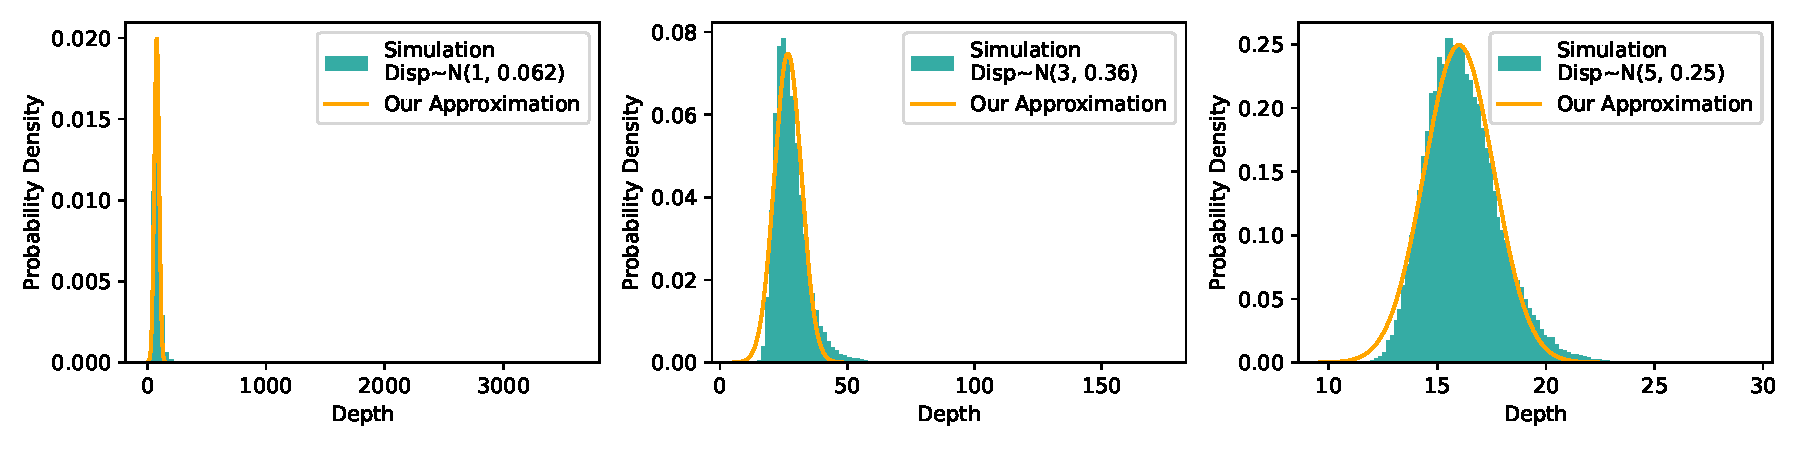
\includegraphics[width=0.8\linewidth]{tex/ch3_macvo/figs/Depth_MonteCarlo.pdf}
    \caption{Result of Monte Carlo simulation on depth distribution. Despite the skewness in the simulated distribution, our approximation matches the simulation. As error rate $\gamma$ increases and average disparity $\Disparity$ approaches $0$ (from right to left), the depth distribution becomes more skewed and the quality of approximation decreases.}
    \label{fig:Montecarlo}
\end{figure}


\subsection{Uncertainty Correction After Keypoint Matching}
\label{sec:macvo:uncertainty_correction}

Let $q_{i, t}$ be the $i$-th keypoint on the camera plane at time $t$. Given the estimated optical flow $\mathbf{f}$ at $q_{i, t}$, the matched keypoint at time $t+1$ is defined as $q_{i, t+1} = q_{i, t} + \mathbf{f}_{i, t}$. Since $\mathbf{f}_{i, t}$ follows the gaussian distribution $\mathcal{N}(\hat{f}_{i, t}, \hat{\Sigma}_{i, t})$, $q_{i, t+1}$ is a random variable following distribution of $\mathcal{N}(q_{i, t} + \hat{f}_{i, t}, \hat{\Sigma}_{i, t})$.

Let $\varphi_{i, t}$ be a 2D Gaussian filter with covariance matrix $\hat{\Sigma}_{i, t}$, the probability for matched keypoint on some pixel $j$ is then expressed as $(\varphi_{i, t})_j$. Let $d_j$ denote the estimated depth at pixel $j$, then the average depth for pixel $q_{i, t+1}$ weighted by $\varphi$ is expressed as
\begin{equation}
    \mu_{d_{i, t}} = \sum_{j}{(\varphi_{i, t})_j \cdot d_j},
\end{equation}
and the estimated variance of depth of $q_{i, t+1}$ is calculated as weighted variance
\begin{equation}
    \sigma_{d_{i, t}}^2 = \sum_j{(\varphi_{i, t})_j \cdot (d_j - \mu_{d_{i, t}})^2}.
\end{equation}
We could also model the depth of the matched point using a mixture of Gaussian distributions, but experiments show that this offers only a minimal performance improvement. Therefore, we use the straightforward weighted variance method to estimate depth uncertainty.

\begin{figure}
    \centering
    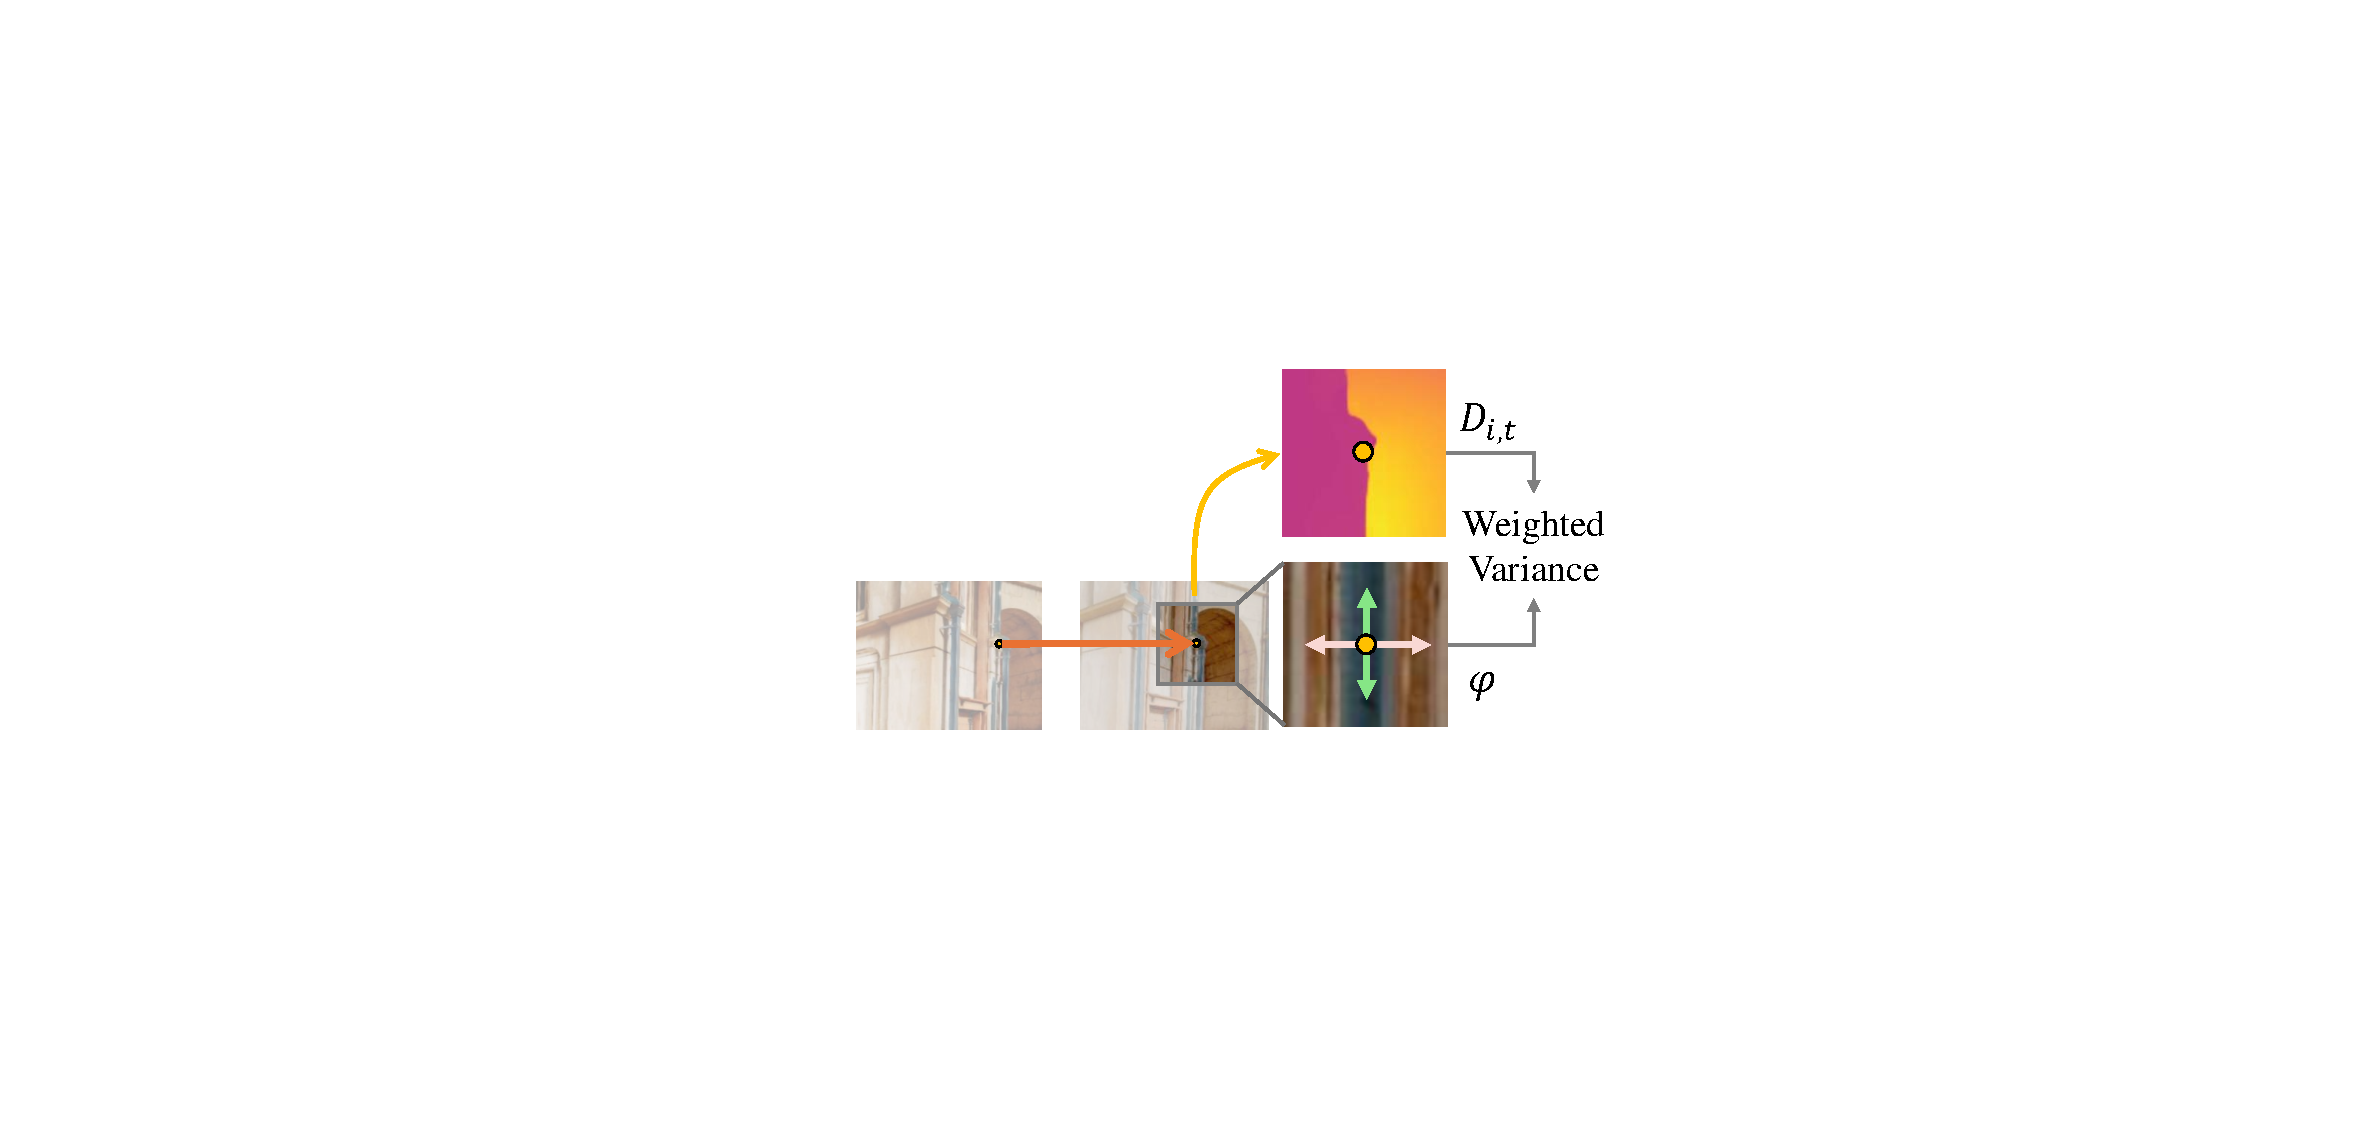
\includegraphics[width=0.7\linewidth]{tex/ch3_macvo/figs/DepthPatchEstimate.pdf}
    \caption{Estimate depth variance of the matched point under the presence of matching uncertainty.}
    \label{fig:depth-patch-estimate-cov}
\end{figure}

\subsection{Projecting 2D Uncertainty to Spatial Covariance}
\label{sec:macvo:Project2DTo3D}

Let $\mathbf{u}_{i, t} \sim \mathcal{N}(u_{i, t}, \sigma_{u_{i, t}}^2)$, $\mathbf{v}_{i, t} \sim \mathcal{N}(v_{i, t}, \sigma_{v_{i, t}}^2)$, and $\mathbf{d}_{i, t} \sim \mathcal{N}(d_{i, t}, \sigma_{d_{i, t}}^2)$, we derive the distribution of 3D point under camera coordinate ${}^c\mathbf{p}_{i, t} = [\mathbf{x}_{i, t}, \mathbf{y}_{i, t}, \mathbf{z}_{i, t}]^\top \sim \mathcal{N}({}^cp_{i, t}, {}^c\Sigma_{i, t})$.

Recall that the relationship between pixel coordinate $(\mathbf{u}_{i, t}, \mathbf{v}_{i, t})$, depth $\mathbf{d}_{i, t}$ and 3D coordinate $\mathbf{x}_{i, t}, \mathbf{y}_{i, t}, \mathbf{z}_{i, t}$ is depicted as
\begin{equation}
    \mathbf{x}_{i, t} = \frac{(\mathbf{u}_{i, t} - c_x)\mathbf{d}_{i, t}}{f_x},\quad \mathbf{y}_{i, t} = \frac{(\mathbf{v}_{i, t} - c_y)\mathbf{d}_{i, t}}{f_y},\quad \mathbf{z}_{i, t} = \mathbf{d}_{i, t}
\end{equation}

Assume $\mathbf{u}_{i, t}$, $\mathbf{v}_{i, t}$, $\mathbf{d}_{i, t}$ are independent to each other, we have $\mathrm{Var}(\mathbf{u}_{i, t}\mathbf{d}_{i, t}) = (\sigma_{u_{i, t}}^2 + d_{i, t}^2)(\sigma_{d_{i, t}}^2 + u_{i, t}^2) - u_{i, t}^2d_{i, t}^2$  \cite{ExactVarianceProduct}. Based on this expression of variance, it follows that
\begin{equation}
\begin{aligned}
    \sigma_{x_{i, t}}^2 &= \mathrm{Var}\left(\frac{(\mathbf{u}_{i, t} - c_x)\mathbf{d}_{i, t}}{f_x} \right) = \frac{\mathrm{Var}((\mathbf{u}_{i, t} - c_x)\mathbf{d}_{i, t})}{f_x^2}\\
        &= \frac{\sigma_{u_{i, t}}^2\sigma_{d_{i, t}}^2 + \sigma_{u_{i, t}}^2\mathbf{d}_{i, t}^2 + (\mathbf{u}_{i, t} - c_x)^2\sigma_{d_{i, t}}^2}{f_x^2}\\
    \sigma_{y_{i, t}}^2 &= \mathrm{Var}\left(\frac{(\mathbf{v}_{i, t} - c_y)\mathbf{d}_{i, t}}{f_y} \right) = \frac{\mathrm{Var}((\mathbf{v}_{i, t} - c_y)\mathbf{d}_{i, t})}{f_y^2}\\
        &= \frac{\sigma_{v_{i, t}}^2\sigma_{d_{i, t}}^2 + \sigma_{v_{i, t}}^2\mathbf{d}_{i, t}^2 + (\mathbf{v}_{i, t} - c_y)^2\sigma_{d_{i, t}}^2}{f_y^2}\\
    \sigma_{z_{i, t}}^2 &= \sigma_{d_{i, t}}^2
\end{aligned}
\end{equation}

Under the assumption that $\mathbf{u}_{i, t}, \mathbf{v}_{i, t}, \mathbf{d}_{i, t}$ are independent to each other, we derive the covariance between $\mathbf{x}_{i, t}$, $\mathbf{y}_{i, t}$ and $\mathbf{z}_{i, t}$ as:
\begin{equation}
    \begin{aligned}
        \mathrm{Cov}(\mathbf{x}_{i, t}, \mathbf{y}_{i, t}) &= \mathrm{Cov}\left(\frac{(\mathbf{u}_{i, t} - c_x)\mathbf{d}_{i, t}}{f_x}, \frac{(\mathbf{v}_{i, t} - c_y)\mathbf{d}_{i, t}}{f_y}\right)\\
            &= \mathbb{E}\left[\frac{\mathbf{d}_{i, t}^2 (\mathbf{u}_{i, t} - c_x) (\mathbf{v}_{i, t} - c_y)}{f_xf_y}\right] \\
            &- \mathbb{E}\left[\frac{(\mathbf{u}_{i, t} - c_x)\mathbf{d}_{i, t}}{f_x}\right]\mathbb{E}\left[\frac{(\mathbf{v}_{i, t} - c_y)\mathbf{d}_{i, t}}{f_y}\right]\\
            &= \frac{(\mathbb{E}[\mathbf{d}_{i, t}^2] - \mathbb{E}[\mathbf{d}_{i, t}]^2)\mathbb{E}[\mathbf{u}_{i, t} - c_x]\mathbb{E}[\mathbf{v}_{i, t} - c_y]}{f_xf_y}\\
            &= \frac{\sigma_{d_{i, t}}^2}{f_xf_y}(u_{i, t} - c_x) (v_{i, t} - c_y)
    \end{aligned}
\end{equation}
and
\begin{equation}
    \begin{aligned}
    \mathrm{Cov}(\mathbf{x}_{i, t}, \mathbf{z}_{i, t}) &= \mathrm{Cov}\left( \frac{(\mathbf{u}_{i, t} - c_x)\mathbf{d}_{i, t}}{f_x}, \mathbf{d}_{i, t} \right) \\
    &= \frac{(\mathbb{E}[\mathbf{d}_{i, t}^2] - \mathbb{E}[\mathbf{d}_{i, t}]^2)\mathbb{E}[\mathbf{u}_{i, t}]}{f_x} = \frac{\sigma_{d_{i, t}}^2}{f_x}(u_{i, t} - c_x)\\
    \mathrm{Cov}(\mathbf{y}_{i, t}, \mathbf{z}_{i, t}) &= \mathrm{Cov}\left( \frac{(\mathbf{v}_{i, t} - c_y)\mathbf{d}_{i, t}}{f_y}, \mathbf{d}_{i,t} \right)\\
    &= \frac{(\mathbb{E}[\mathbf{d}_{i, t}^2] - \mathbb{E}[\mathbf{d}_{i, t}]^2)\mathbb{E}[\mathbf{v}_{i, t}]}{f_y} = \frac{\sigma_{d_{i, t}}^2}{f_y}(v_{i, t} - c_y)
    \end{aligned}
\end{equation}

\fref{fig: DiagonalCovarianceVisualization} visualizes the distribution of keypoints in 3D space via Monte Carlo and the 90\% confidence interval of estimated distribution, confirming the necessity of off-diagonal terms.

\begin{figure}[h!]
    \centering
    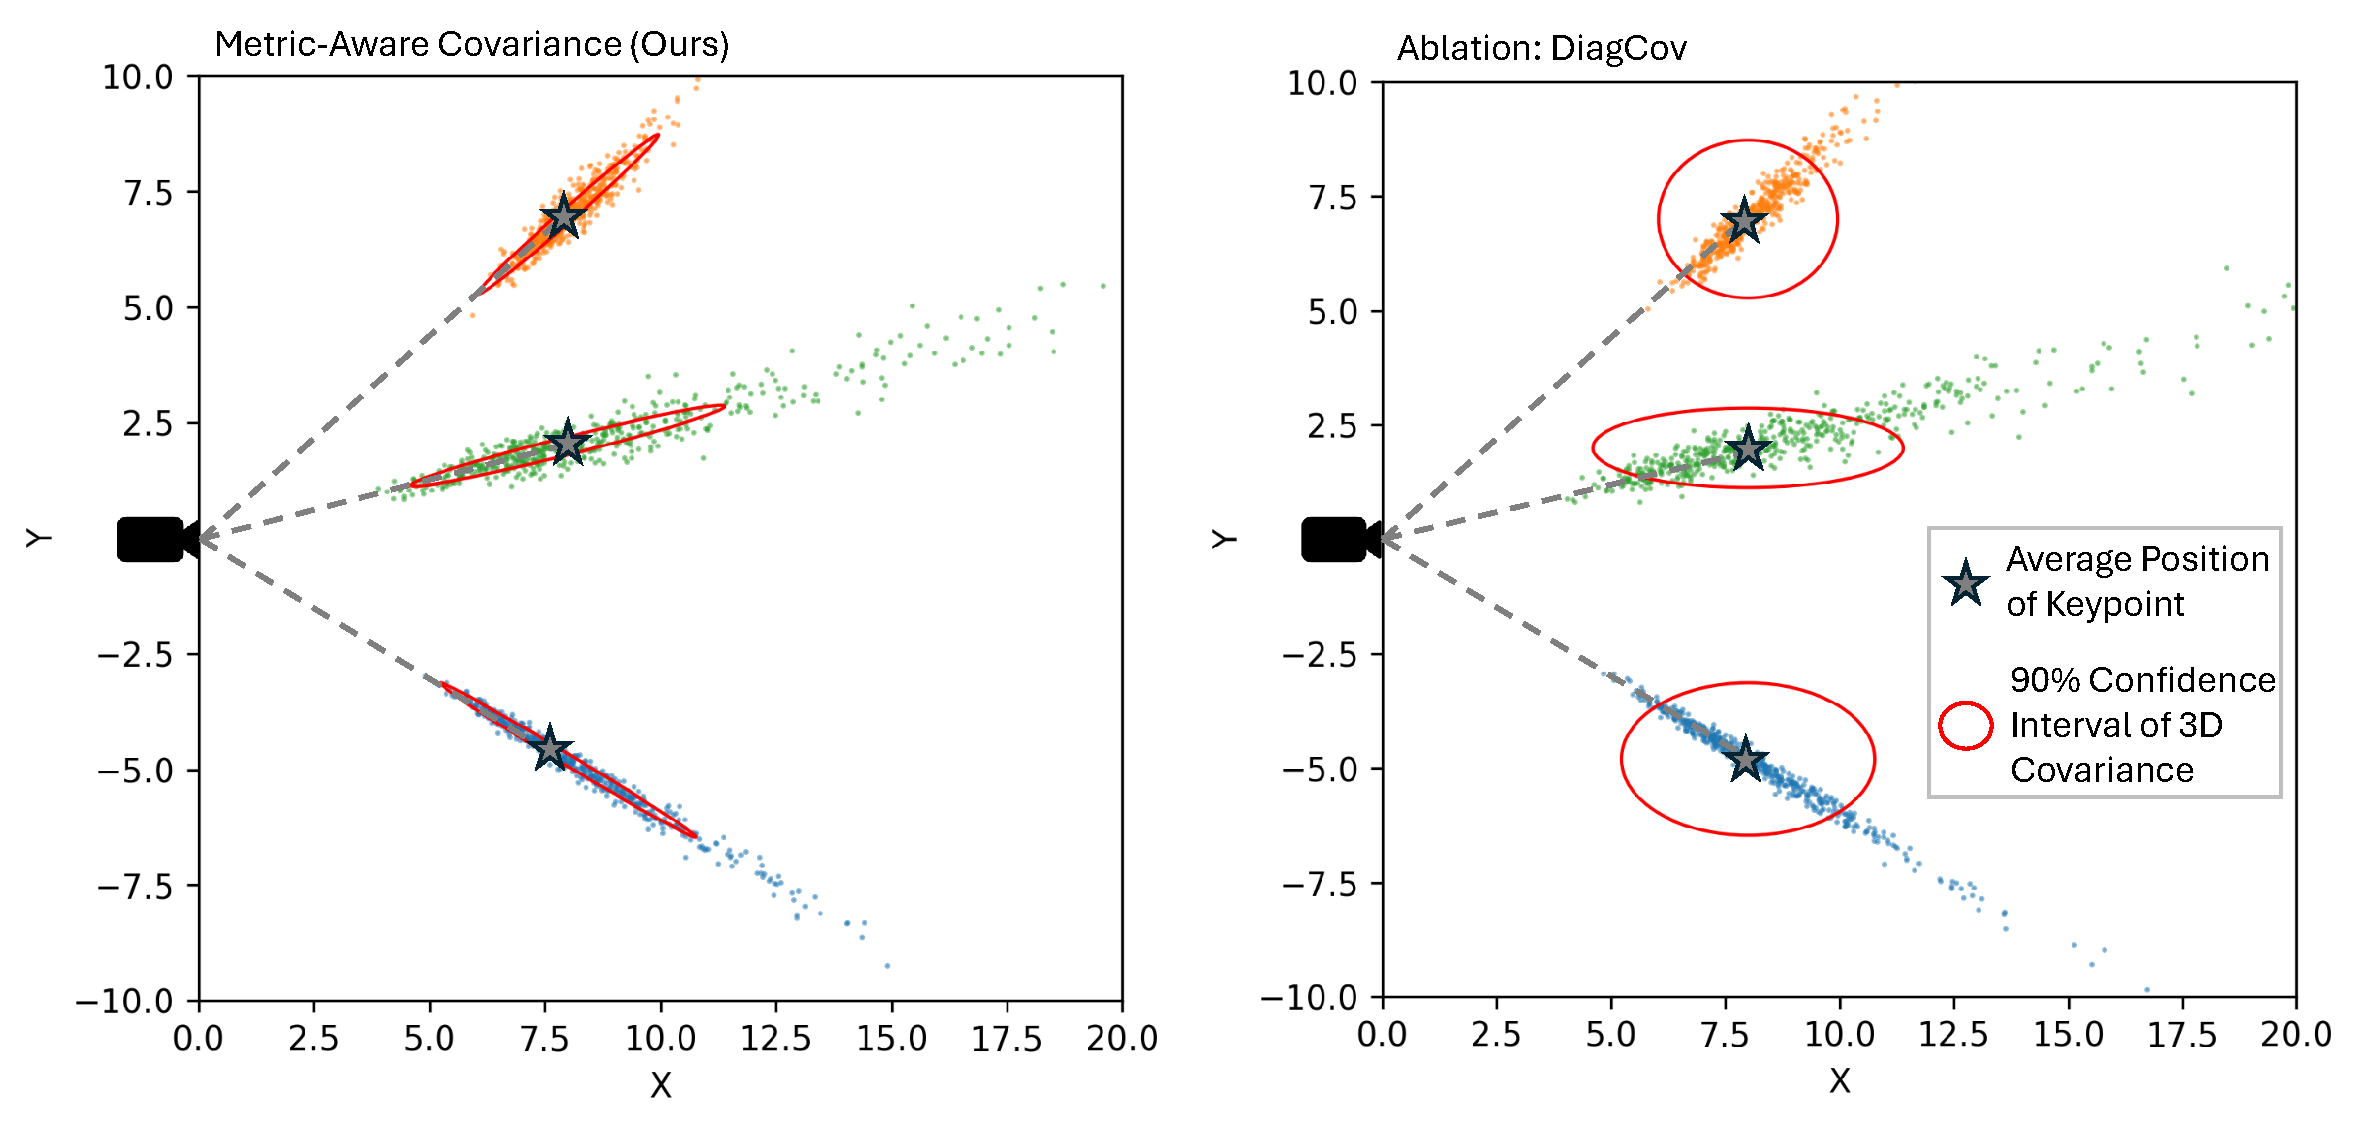
\includegraphics[width=0.8\linewidth]{tex/ch3_macvo/figs/CovModelAblation.pdf}
    \caption{Comparison of proposed 3D covariance (\textbf{left}) and the diagonal covariance matrix (\textbf{right}, DiagCov in ablation study). Our method captures the uncertainty of keypoints significantly better than the diagonal covariance matrix.}
    \label{fig: DiagonalCovarianceVisualization}
\end{figure}


\section{Runtime Analysis Details}
\label{sec:macvo:RuntimeAnalysis}

\begin{figure}[t]
    \centering
    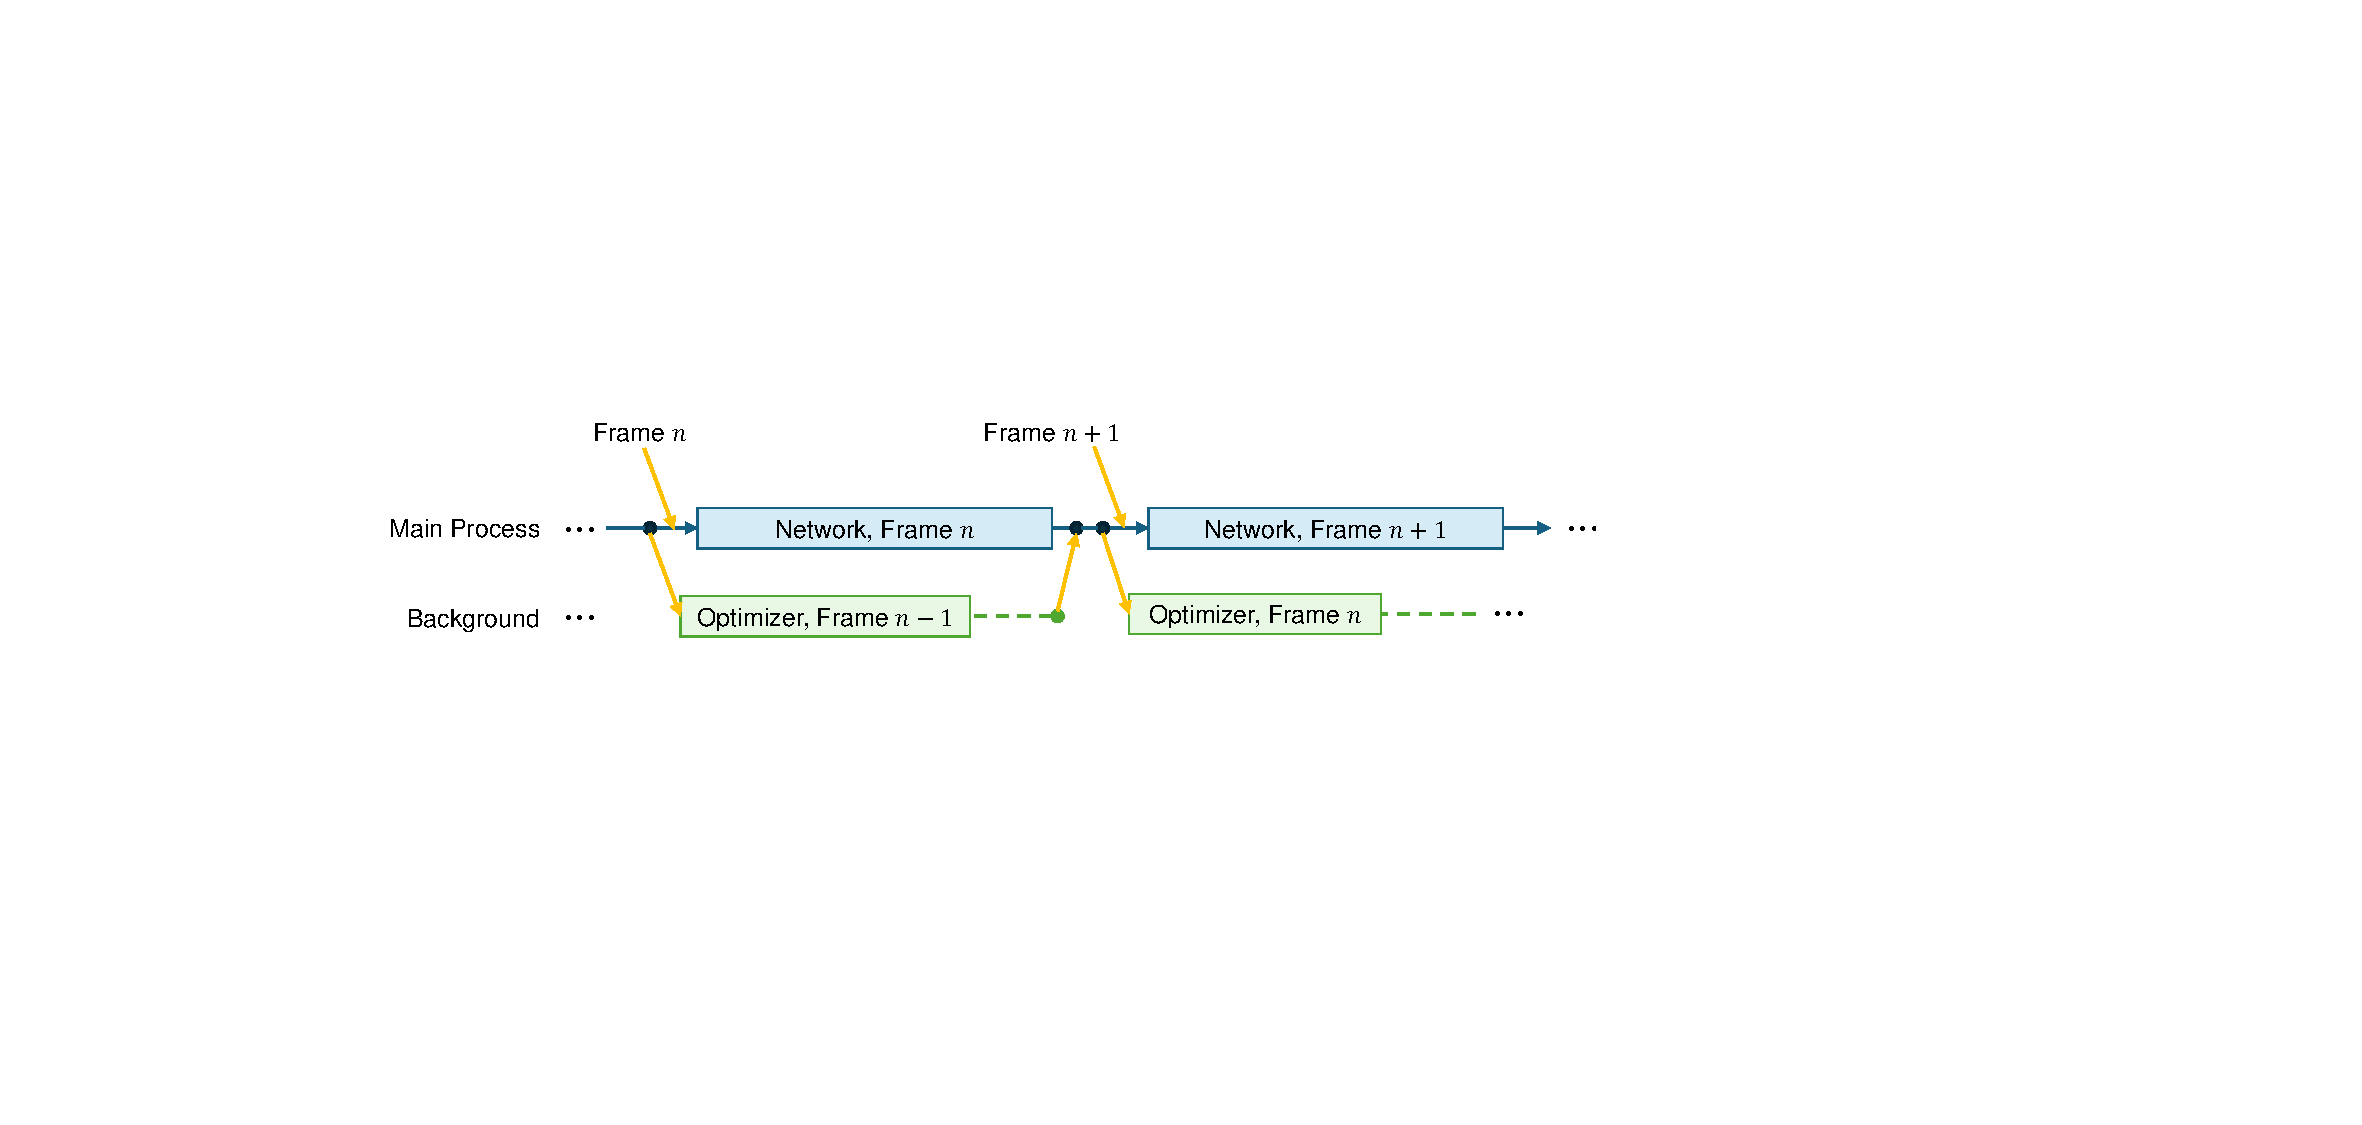
\includegraphics[width=0.8\linewidth]{tex/ch3_macvo/figs/MultiprocessPipeline.pdf}
    \caption{Multiprocessing setup places the optimizer in the background process and parallelizes the CPU-intensive (optimizer) and GPU-intensive (frontend network inference) jobs.}
    \label{fig: multiprocesspipeline}
\end{figure}

The runtime analysis uses the platform with \texttt{AMD Ryzen 9 5950X} CPU and \texttt{NVIDIA 3090 Ti} GPU.
To speed up the frontend network, we utilize  TensorRT (\textbf{TRT}), and multi-processing (\textbf{MP}) to accelerate the original network (\textbf{Raw}).
In our multiprocessing setup, as shown in \fref{fig: multiprocesspipeline}, a new CPU process is initiated to run the pose graph optimization in parallel with the front-end network, thereby maximizing GPU utilization.

We also introduce a fast mode (\textbf{MAC-VO Fast}) which utilizes half-precision (\texttt{bfloat16}) number in the network inference to enhance computational efficiency.
This mode also speeds up the memory decoder network by reducing the number of iterative updates from 12 to 4. 
The fast mode performs \textbf{10.5 fps} (frames per second) with 70\% of the performance of the original MAC-VO. 


\section{Datasets and Implementation Details}

\paragraph{TartanAir dataset}
The TartanAir dataset is a large-scale synthetic dataset encompassing highly diverse scenes, including various complex and challenging environments. 
Following the TartanAir data generation method, we created new, more diverse and challenging trajectories. 
From these, we selected that feature fast camera movements, low-light indoor environments, and simulated lunar surfaces lacking visual features. The images in the new dataset have a resolution of \(640 \times 640\). 
When testing iSLAM-VO and TartanVO, we resized the input images to \(448 \times 640\) to match the input requirements of the optical flow network. Due to the substantial GPU memory required by DROID-SLAM for global bundle adjustment optimization when processing high-resolution images, we reduced the input image resolution to \(512 \times 512 \) and manually reclaimed GPU and memory after testing each trajectory to avoid potential memory insufficiency.

\paragraph{KITTI dataset}
The KITTI dataset is a well-known and widely used dataset for autonomous driving, containing detailed ground truth labels that make it suitable for evaluating the performance of various VO/SLAM methods. 
Learning-based methods may experience performance degradation when handling the image sizes in the KITTI dataset, therefore, we cropped the input images to different sizes based on the methods tested. Our model processed images cropped to \( 376\times680\), while for testing DROID-SLAM, the images were cropped to \( 320 \times 832\).

\paragraph{EuRoC dataset}
 The EuRoC dataset consists of 11 trajectories collected by a drone and is also a widely used benchmark for VO/SLAM tasks. Some scenes in this dataset contain thousands of image pairs, which imposes computational pressure on DROID-SLAM when performing bundle adjustment. Thus, during testing, we reduced the input image resolution to \( 320 \times 512\) and read every other frame of image pairs. In post-processing, we completed the entire trajectory by interpolating timestamps.

\paragraph{ZED Camera data}
The ZED Camera data comprises real-world trajectory data captured using a ZED stereo camera, employed to test the robustness and generality of our model when faced with unseen data not present in the training set.
